\section{Control}
\label{sec:control}
Control is the VHDL component that acts as top module of this project. 
It contains the components described in previous sections and connects them.
This is also where the sorting of the bricks is done.
\begin{figure}[h!]
	\centering
	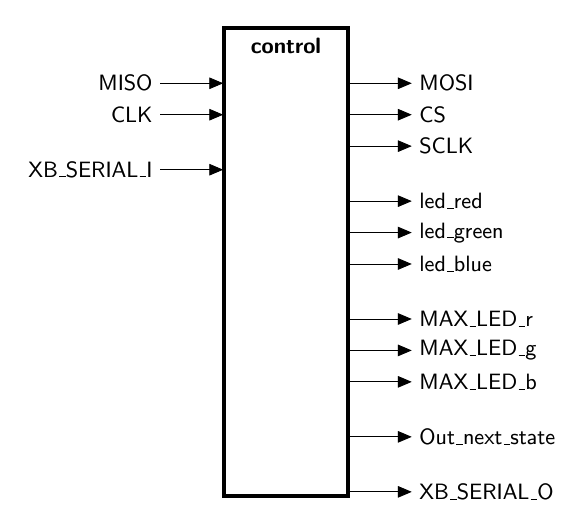
\includegraphics[scale=0.4]{images/ent_control}
	\caption{Pinout of the control component.}
	\label{fig:pinoutcontrol}
\end{figure}
Control makes 10 readings from the reflection of each colour, 30 readings in total. 
At the end the flipper is moved to either the left or right position, based on the 30 readings that were performed.

\subsection{Implementation of Control}

%Image of the full design

Control has  one process named \texttt{readBlock} which determines the colour of the block of the block. \\

%It start by setting \texttt{led\_on} high.  %Hvorfor gjorde jeg det.. Ikke nødvendigt... 

The process starts signalling the component \texttt{LED\_driver} to turn on the red LED. 
After 13$\mu$s the \texttt{LED\_driver} sets \texttt{start\_adc} high. 
When the ADC component reads \texttt{start\_adc} as high it will start converting the voltage from the photodiode.  
When the voltage is, it will set \texttt{read\_adc} high. 
When control reads \texttt{read\_adc} as high it will read the 10 bit value output on \texttt{ADC\_value}. When the the binary value has been intepreted, either \texttt{redCount}, \texttt{blueCount} or \texttt{greenCount} is incremented, depending on the colour that passed the photodiode.
Now, \texttt{adc\_read} is set high. This signals the LED driver to change its state to the next state.

After 30 iterations, the counter, \texttt{redCount}, \texttt{blueCount} and \texttt{greenCount}, with the highest value will dictate which position the servo motor will move to.
This "voting system" will minimize the effect of failed readings.

